\documentclass[12pt]{article}   % use documentclass amsart too if you want
\usepackage{amsmath,amsthm,amssymb}
\usepackage[margin=1in]{geometry}
\usepackage{color}
\usepackage{hyperref}
\usepackage{graphicx}
\usepackage{fancyhdr} % COMMENT THIS OUT TO TURN OFF FANCY HEADERS
\usepackage{verbatim}

\hypersetup{
  colorlinks= true, %Colours links instead of ugly boxes
  urlcolor   = blue, %Colour for external hyperlinks
  linkcolor  = blue, %Colour of internal links
  citecolor  = blue %Colour of citations
}





\newtheorem{theorem}[equation]{Theorem}
\newtheorem{lemma}[equation]{Lemma}
\newtheorem{corollary}[equation]{Corollary}
\theoremstyle{definition}
\newtheorem{exercise}[equation]{Exercise}

\newtheorem{example}[equation]{Example}
\newtheorem{definition}[equation]{Definition}
\newtheorem{question}[equation]{Question}
\newtheorem{remark}[equation]{Remark}

\numberwithin{equation}{section}

%@@@@@@@@@@@@@@@@@@@@@@@@@@@@@@@@@@@@@@@@@@@@@@@@@@@@@@@@@@@@@@@@@@@@@@@@@@@@@@@@@@@@@@@@@

\begin{document}
\parskip10pt
\parindent0pt
\baselineskip15pt



\title{APPM 2360 PROJECT 3: THE LOTKA-VOLTERRA PREDATOR PREY MODEL}
\author{Ethan Burkley (section 251), \\ Davis Landry (section 213), Max Morgan (section 244)}


\pagestyle{fancy}
\renewcommand{\sectionmark}[1]{\markright{#1}{}}

\fancyhf{}

\rhead{\fancyplain{}{\thepage}} % predefined ()
\lhead{\fancyplain{}{\rightmark }} % 1. sectionname, 1.1 subsection name etc
%\cfoot{\fancyplain{}{\thepage}}

\maketitle

%@@@@@@@@@@@@@@@@@@@@@@@@@@@@@@@@@@@@@@@@@@@@@@@@@@@@@@@@@@@@@@@@@@@@@@@@@@@@@@@@@@@@@@@@@
\newpage
\setcounter{page}{2}
\section{Introduction} \label{APPM2360proj01sec01}
\quad Understanding the growth of a population is a complex challenge as population dynamics depend on a large number of factors such as fertility, size, and available resources. Understanding the growth of a population becomes more complicated when observing the biological system of two interacting species.There are many ways to model the relationship between the populations of a species of predator and prey. The populations of predators and prey are interdependent, however the size of one population causes spikes or dips in the other. Beyond just the size of the species' populations, there are many external factors that can influence the growth of these species. Including these into the model results in more accurate, yet more complex, models. More intricate models take into account factors found in populations such as carrying capacity and migration in order to better predict the future growth or decline of populations. The Lotka-Volterra model incorporates observational data of a species' growth and the rate of interactions between species in order to understand the dynamics of population of predators and prey. 
 
%@@@@@@@@@@@@@@@@@@@@@@@@@@@@@@@@@@@@@@@@@@@@@@@@@@@@@@@@@@@@@@@@@@@@@@@@@@@@@@@@@@@@@@@@
\setcounter{page}{3}
\section{Background} \label{APPM2360proj01sec01}
\quad A simplified population growth model assumes that the growth rate of the population $\frac{dP}{dt}$ is proportional to the current size of the of population $P$. This yields the differential equation $\frac{dP}{dt}=rP$, where $r$ is the intrinsic growth rate of the population. However, the model must be adjusted when considering the dynamics of a predator species interacting with a prey species. Both the populations will still grow proportionally to their size, but now the size of the other population must also be taken into consideration. The predator species population, with morality rate $a$, is supported by interactions with the prey species. The constant $b$ represents the reproduction rate of predator per prey. Therefore the predator population grows according to the following differential equation, 
\begin{align*}
%
\frac{dx_1}{dt} & = -ax_1 + bx_1x_2 ,\ x_1(0) = x_{1,0}\\
%
\end{align*}
where $x_{1,0}$ is the experimentally observed initial size of predator population. 

\quad The prey population grows according to the simplified population growth model, where the population growth rate is proportional to the population size. The constant $c$ represents the reproduction rate of the prey. Because the predator population hunts prey, population is negatively impacted by these interactions. The constant $d$ mortality rate of predator per prey. Therefore the prey population grows according to the following differential equation,
\begin{align*}
%
\frac{dx_2}{dt} & = cx_1 - dx_1x_2 ,\ x_2(0) = x_{2,0}\\
%
\end{align*}
where $x_{2,0}$ is the experimentally observed initial size of prey population. 

The Lotka-Volterra predator prey model uses the coupled system of differential equations to describe the dynamics of the two species' populations. The function $x_1(t)$ describes the size of the predator population with respect to time and the function $x_2(t)$ describes the prey population with respect to time. 

%@@@@@@@@@@@@@@@@@@@@@@@@@@@@@@@@@@@@@@@@@@@@@@@@@@@@@@@@@@@@@@@@@@@@@@@@@@@@@@@@@@@@@@@@
\setcounter{page}{4}
\section{Problem Statement} \label{APPM2360proj01sec01}




%@@@@@@@@@@@@@@@@@@@@@@@@@@@@@@@@@@@@@@@@@@@@@@@@@@@@@@@@@@@@@@@@@@@@@@@@@@@@@@@@@@@@@@@@
\setcounter{page}{5}
\section{Calculations and Results} \label{APPM2360proj01sec01} 

From here, the horizontal and vertical nullclines are determined by setting the $\frac{dx_1}{dt}$ and $\frac{dx_2}{dt}$ equal to zero. Conceptually, when $\frac{dx_1}{dt}$ is equal to 0, there is no change along the horizontal axis and when $\frac{dx_2}{dt}$ is equal to 0, there is no change along the vertical axis. 
\begin{align*}
& \frac{dx_1}{dt} = \frac{dx_2}{dt} = 0
\end{align*}

Therefore the vertical nullclines are,
\begin{align*}
%
0 & =  -ax_1 + bx_1x_2 \\
%  
 & = x_1(-a + bx_2) \\
%
x_1 &= 0, \ x_2 = \frac{a}{b}  
%
\end{align*}
And the horizontal nullclines are, 
\begin{align*}
%
0 & = cx_2 - dx_1x_2 \\  
%
& =  x_2(c - dx_1) \\
%
x_2 &= 0, \ x_1 = \frac{c}{d} 
\end{align*}



The two-dimensional system of autonomous, first order differential equations can be written in matrix vector form as a vector valued function, 
\begin{align*} 
\textbf{x}'(t) 
= 
\begin{bmatrix}
     -ax_1 + bx_1x_2\\
     cx_2 - dx_1x_2\\
\end{bmatrix}
\end{align*}

The Jacobian matrix for this system is give by
\begin{align*} 
J 
=
\begin{bmatrix}
     \frac{\partial{x'_1}}{\partial{x_1}} & \frac{\partial{x'_1}}{\partial{x_2}}\\
     \frac{\partial{x'_2}}{\partial{x_1}} &  \frac{\partial{x'_2}}{\partial{x_2}}\\
\end{bmatrix}
=
\begin{bmatrix}
     -a+bx_2 & bx_1\\
     -dx_2 & c-dx_1\\
\end{bmatrix}
\end{align*}

\quad Now, the stability of the equilibrium solutions of the system of differential equations can be determined by using the eigenvalues of the Jacobian matrix. The Equilibrium points are at the intersections of the vertical nullcline and the horizontal nullcline, $(0,0)$ and $(\frac{c}{d},\frac{a}{b})$.  

For the equilibrium point $(0,0)$ we get $\lambda=-a,\ c$, which is unstable.
\begin{align*}
\begin{vmatrix}
	-a-\lambda &0\\
	0& c-\lambda\\
\end{vmatrix}
=(-a-\lambda)(c-\lambda)
\end{align*}

For the equilibrium point $(\frac{c}{d},\frac{a}{b})$ we get $\lambda=\pm\sqrt{-ac}$, which is neutrally stable.
\begin{align*}
\begin{vmatrix}
	0-\lambda & \frac{bc}{d}\\
	\frac{-da}{b} & 0-\lambda\\
\end{vmatrix}
=\lambda^2+ac
\end{align*}

\quad The physical interpretation of $(0,0)$ being unstable is that if any prey exist in this system then they will move away from the equilibrium point. The point $(\frac{c}{d},\frac{a}{b})$ is neutrally stable which means that once there the populations will oscillate around that point. 
\begin{comment}
\begin{figure}
	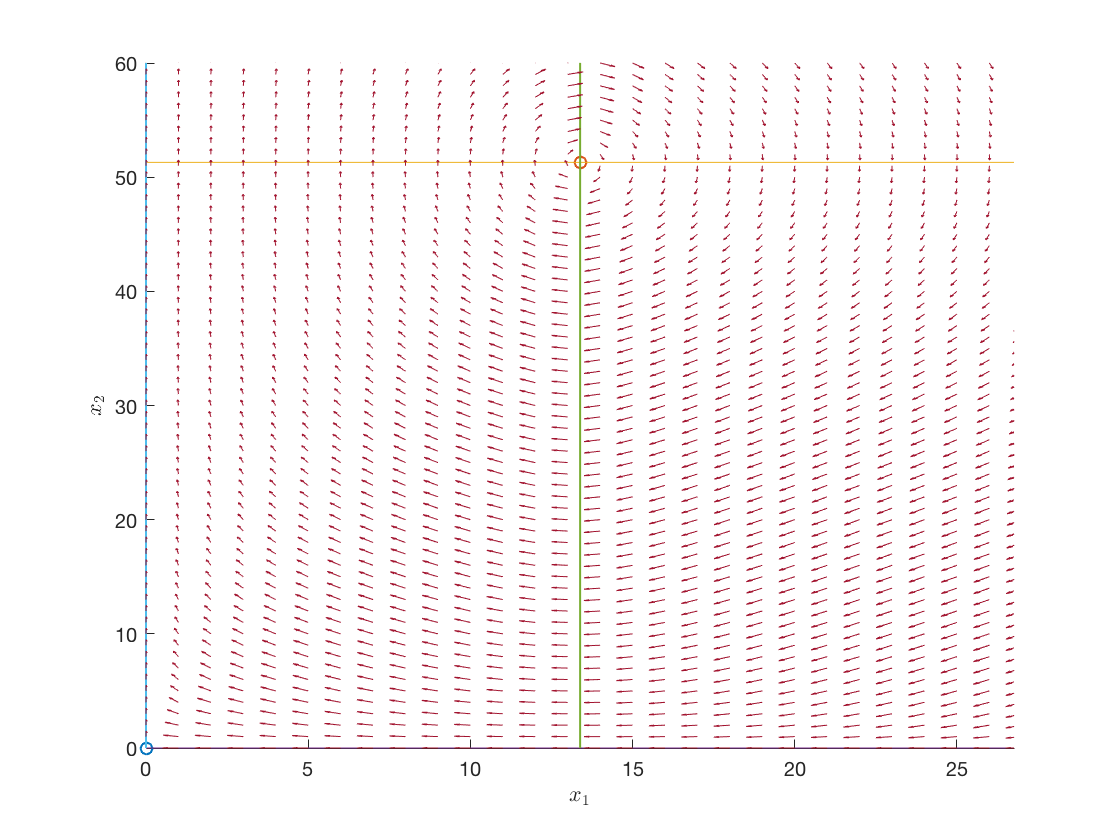
\includegraphics[width=\lindwidth]{dirfield.png}
	\caption{Direction Field Plot}
	\label{fig:dirfield}
\end{figure}
\end{comment}

%@@@@@@@@@@@@@@@@@@@@@@@@@@@@@@@@@@@@@@@@@@@@@@@@@@@@@@@@@@@@@@@@@@@@@@@@@@@@@@@@@@@@@@@@
\setcounter{page}{6}
\section{Conclusion} \label{APPM2360proj01sec01}
\quad As the predator species grows, there will by more interactions with the prey species. This will have the effect of decreasing the size of the prey population as more predators hunt for food. A smaller prey population will in turn decrease the predator population by causing a food shortage. This decrease in the predator population ultimately allows the prey population to rebound and increase again.This balanced cycle repeats as time moves forward.    



%@@@@@@@@@@@@@@@@@@@@@@@@@@@@@@@@@@@@@@@@@@@@@@@@@@@@@@@@@@@@@@@@@@@@@@@@@@@@@@@@@@@@@@@@
\newpage
\setcounter{page}{7}
\section{Appendix} \label{APPM2360proj01sec01}

\end{document} 